\documentclass{ctexart}
\title{hello LaTeX}
\author{ Mary\thanks{E-mail:*****@***.com}
\and Ted\thanks{Corresponding author}
\and Louis}
\date{\today}
\usepackage{array}
\usepackage{tabularx}
\usepackage{booktabs}
\usepackage{multirow}
\usepackage{makecell}
\usepackage{graphicx}

\begin{document}

\begin{titlepage}
    \maketitle
\end{titlepage}

\newpage

\tableofcontents
\newpage


\section{section one title}
\paragraph{star paragraph}

here\label{sec:this} some explaints about `this' ...

\newpage

% 手动添加
\addcontentsline{toc}{section}{manual add title}

\section{section two title}
\paragraph{paragraph}
A reference to this subsection `this' looks like: ``see section~\ref{sec:this} on page~\pageref{sec:this}.''

bookmark\footnote{12345} ...
\marginpar{\footnotesize 边注较窄,不要写过多文字,最好设置较小的字号。}

\section{特殊环境}

\subsection*{列表}

\begin{enumerate}
    \item An item.
          \begin{enumerate}
              \item A nested item.\label{itref}
              \item[*] A starred item.
          \end{enumerate}
    \item Reference(\ref{itref}).
\end{enumerate}

\renewcommand{\labelenumi}{\Alph{enumi}>}
\begin{enumerate}
    \item First item
    \item Second item
\end{enumerate}

\subsection*{对齐环境}

\begin{center}
    Centered text using a
    \verb|center| environment.
\end{center}
\begin{flushleft}
    Left-aligned text using a
    \verb|flushleft| environment.
\end{flushleft}
\begin{flushright}
    Right-aligned text using a
    \verb|flushright| environment.
\end{flushright}

% \centering
% aaaa

\subsection*{代码环境}

\begin{verbatim}
    #include <iostream>
    int main()
    {
    std::cout << "Hello, world!"
    << std::endl;
    return 0;
    }
\end{verbatim}

\verb|\LaTeX|
\verb+(a || b)+ \verb*+(a || b)+

\subsection*{表格}

\begin{tabular}{|l|c|r|}
    \hline
    left & center & right \\
    \hline
\end{tabular}
\\[10pt]

\begin{tabular}{@{} r@{:}lr @{}}
    \hline
    1  & 1 & one    \\
    11 & 3 & eleven \\
    \hline
\end{tabular}
\\[10pt]

\begin{tabular}{r@{:}lr}
    \hline
    1  & 1 & one    \\
    11 & 3 & eleven \\
    \hline
\end{tabular}
\\[10pt]

\begin{tabular}{rlr}
    \hline
    1  & 1 & one    \\
    11 & 3 & eleven \\
    \hline
\end{tabular}
\\[10pt]

\begin{tabular}{>{\itshape}r<{\&}l}
    \hline
    italic & normal \\
    column & column \\
    \hline
\end{tabular}
\\[1em]

\newcommand\txt
{a b c d e f g h i}
\begin{tabular}{cp{2em}m{2em}p{2em}}
    \hline
    pos & \txt & \txt & \txt \\
    \hline
\end{tabular}
\\[1em]

\begin{tabular*}{14em}%
    {@{\extracolsep{\fill}}|c|c|c|c|}
    \hline
    A & B & C & D \\ \hline
    a & b & c & d \\ \hline
\end{tabular*}
\\[1em]

\begin{tabularx}{18em}%
    {|*{4}{>{\centering\arraybackslash}X|}}
    \hline
    A & B & C & D43241 \\ \hline
    a & b & c & d      \\ \hline
\end{tabularx}
\\[1em]

\begin{tabular}{|c|c|c|}
    \hline
    1 & 2 & 3 \\ \cline{1-2}
    4 & 5 & 6 \\ \cline{3-3}
    7 & 8 & 9 \\ \hline
\end{tabular}
\\[1em]

\begin{tabular}{cccc}
    \toprule
             & \multicolumn{3}{c}{Numbers}            \\
    \cmidrule{2-4}
             & 1                           & 2  & 3   \\
    \midrule
    Alphabet & A                           & B  & C   \\
    Roman    & I                           & II & III \\
    \bottomrule
\end{tabular}
\\[1em]

\begin{tabular}{|c|c|c|}
    \hline
    1                      & 2                          & Center \\ \hline
    \multicolumn{2}{c|}{3} & \multicolumn{1}{r|}{Right}          \\ \hline
    4                      & \multicolumn{2}{c|}{C}              \\ \hline
\end{tabular}
\\[1em]

\begin{tabular}{ccc}
    \hline
    \multirow{2}{*}{Item} & \multicolumn{2}{c}{Value}          \\ \cline{2-3}
                          & First                     & Second \\ \hline
    A                     & 1                         & 2      \\ \hline
\end{tabular}
\\[1em]

\begin{tabular}{|c|c|}
    \hline
    a & \makecell{d1 \\ d2} \\
    \hline
    b & c            \\
    \hline
\end{tabular}
\\ [2em]

% \renewcommand\arraystretch{1.8}
\begin{tabular}{|c|}
    \hline
    Really loose  \\ \hline
    tabular rows. \\ \hline
\end{tabular}
\\[1em]

\begin{tabular}{c}
    Head lines    \\ [6pt]
    tabular lines \\ [6pt]
    tabular lines \\ \hline
\end{tabular}
\\ [1em]

\section*{图片}

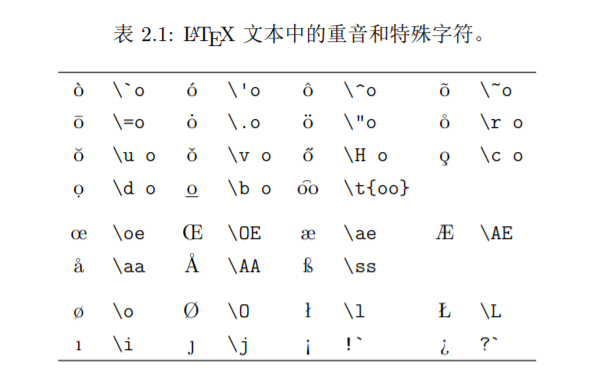
\includegraphics[scale=1.2]{LaTeX文本中的重音和特殊字符.png}

\end{document}
